\documentclass[UTF8,12pt]{article} % 12pt 为字号大小
\usepackage{amssymb,amsfonts,amsmath,amsthm}
\usepackage{times}
\usepackage{graphicx} % 插图
\usepackage{cite}
\usepackage{xeCJK}
\usepackage{color}
\usepackage{caption}
\usepackage{placeins} % 防止浮动
\usepackage{listings}
\lstset{
 columns=fixed,       
 numbers=left,                                        % 在左侧显示行号
 numberstyle=\tiny\color{gray},                       % 设定行号格式
 frame=none,                                          % 不显示背景边框
 backgroundcolor=\color[RGB]{245,245,244},            % 设定背景颜色
 keywordstyle=\color[RGB]{40,40,255},                 % 设定关键字颜色
 numberstyle=\footnotesize\color{darkgray},           
 commentstyle=\it\color[RGB]{0,96,96},                % 设置代码注释的格式
 stringstyle=\rmfamily\slshape\color[RGB]{128,0,0},   % 设置字符串格式
 showstringspaces=false,                              % 不显示字符串中的空格
 language=c++,                                        % 设置语言
}
\usepackage{algorithm}  
\usepackage{algpseudocode}  
\usepackage{amsmath}  
\renewcommand{\algorithmicrequire}{\textbf{Input:}}  
\renewcommand{\algorithmicensure}{\textbf{Output:}} 

\newcommand*{\songti}{\CJKfamily{zhsong}} % 宋体
\newcommand*{\heiti}{\CJKfamily{zhhei}}   % 黑体
\newcommand*{\kaiti}{\CJKfamily{zhkai}}  % 楷体
\newcommand*{\fangsong}{\CJKfamily{zhfs}} % 仿宋
\newcommand*{\lishu}{\CJKfamily{zhli}}    % 隶书
\newcommand*{\yuanti}{\CJKfamily{zhyou}} % 圆体

\usepackage{indentfirst}
\setlength{\parindent}{2em}
\renewcommand{\baselinestretch}{1.25} % 1.25倍行距
\usepackage[a4paper]{geometry}
\geometry{verbose,
  tmargin=2cm,% 上边距
  bmargin=2cm,% 下边距
  lmargin=2cm,% 左边距
  rmargin=2cm % 右边距
}

\usepackage{titlesec} 
\titleformat{\section}[block]{\large \bfseries}{\arabic{section}}{1em}{}[]
\titleformat{\subsection}[block]{\normalsize \bfseries}{\arabic{section}.\arabic{subsection}}{1em}{}[]
\titleformat{\subsubsection}[block]{\small \mdseries}{\arabic{section}.\arabic{subsection}.\arabic{subsubsection}}{1em}{}[]
\titleformat{\paragraph}[block]{\footnotesize \bfseries}{[\arabic{paragraph}]}{1em}{}[]

\usepackage[x11names]{xcolor} 
\usepackage{graphicx}
\usepackage{pstricks,pst-plot,pst-eps}
\usepackage{subfig}
\def\pgfsysdriver{pgfsys-dvipdfmx.def} 
\usepackage{tikz}
\usepackage{verbatim}
\usepackage[colorlinks,linkcolor=red]{hyperref}
\usepackage{tabularx}

\captionsetup[figure]{labelsep=period}
\captionsetup[table]{labelsep=period}

\begin{document}
\renewcommand{\figurename}{图}
\renewcommand{\tablename}{表}
\renewcommand{\refname}{参考文献}

\title{\bf{\heiti 计算机前沿技术成果复现计划}}
\author{\normalsize{姓名: 徐吕恒}\hspace{2cm}\normalsize{学号: 2410105005}}
\date{}
\maketitle


\section{拟复现原文}

\textbf{A Recurrent Network Model of Planning Explains Hippocampal Replay and Human Behavior(2024 Nature Neuroscience)}

\textbf{\textcolor[rgb]{1,0,0}{原文提供了Julia的源代码,本人使用Python复现}}

\subsection{论文主要内容概述}

该论文提出了一种递归网络模型,用于解释海马体重放和人类行为。通过模拟实验,展示了该模型在不同任务中的表现。具体来说,论文的主要内容包括:

\begin{itemize}
    \item 提出了一种递归网络模型,该模型通过前额叶皮层控制规划过程。
    \item 模型包括一个元强化学习代理,能够通过采样想象的动作序列(称为“rollouts”)来进行规划。
    \item 在空间导航任务中,代理学习在有益的情况下进行规划,为人类思考时间的变异性提供了规范解释。
    \item 人工代理使用的策略rollouts模式与啮齿动物海马体重放模式高度相似。
    \item 该工作提供了一种理论,解释了大脑如何通过前额叶-海马体相互作用实现规划,其中海马体重放由前额叶动态触发并适应性地影响前额叶动态。
\end{itemize}

\begin{figure}[ht]
  \centering
  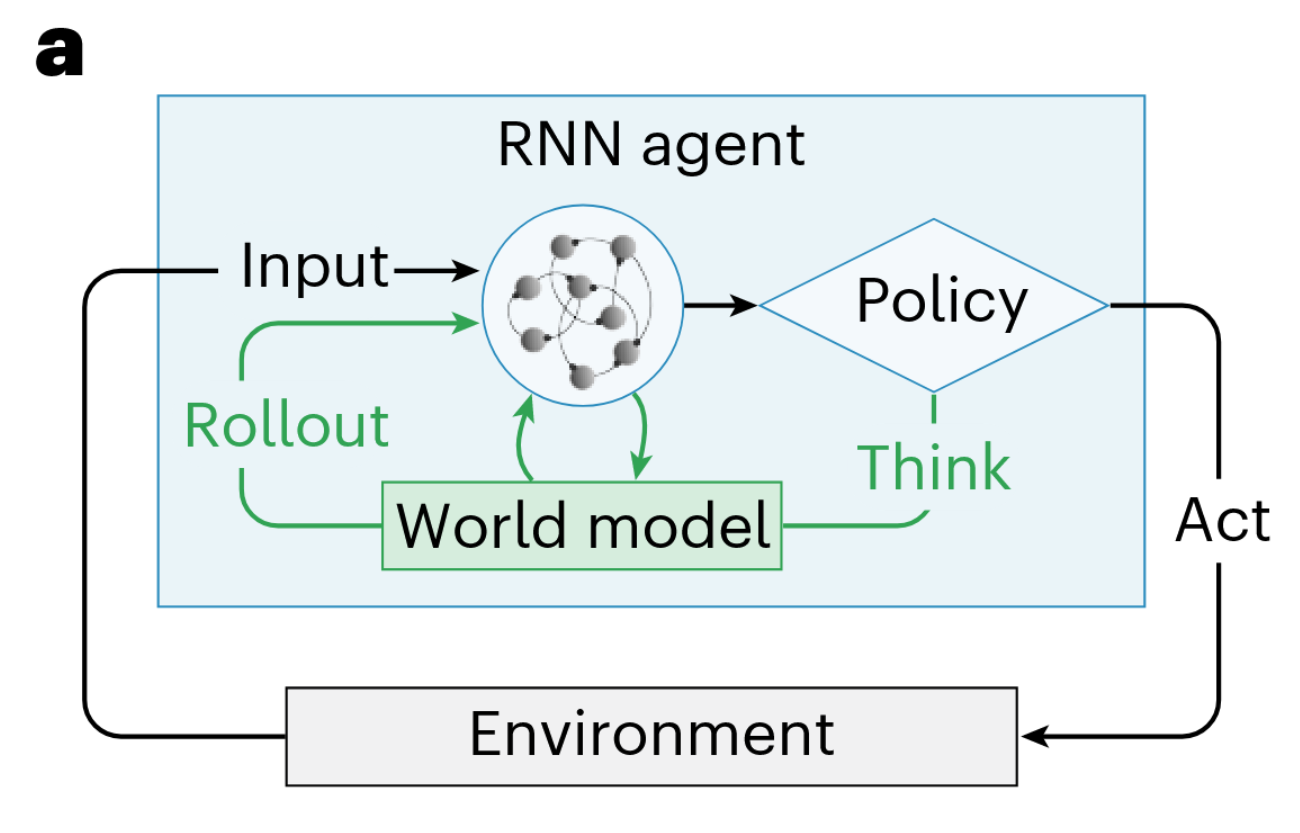
\includegraphics[scale=0.2]{figs/fig2.png}
  \captionsetup{font={scriptsize,stretch=1}}
  \caption{Agent结构示意图。}
  \label{fig:Agent-model}
\end{figure}

\subsection{论文主要技术创新点}

\begin{itemize}
    \item 提出了新的递归网络模型,该模型结合了慢速的突触学习和快速的前额叶网络适应性。
    \item 模型能够解释海马体重放现象,并通过内部世界模型生成与环境交互的想象动作序列。
    \item 模型在空间导航任务中,能够快速适应新环境并优化决策过程。
\end{itemize}

\section{复现工作说明}

\subsection{选择理由}

该论文提出的模型具有重要的理论和实际意义,复现该模型有助于深入理解其工作原理和应用潜力。具体理由包括:

\begin{itemize}
    \item 该模型提供了一种新的视角来理解人类和动物的规划行为。
    \item 通过复现该模型,可以验证其在不同任务中的泛化能力和鲁棒性。
    \item 该模型的复现可以为未来的研究提供基础,探索其在更广泛的应用场景中的潜力。
\end{itemize}

\subsection{拟复现的具体内容}

\begin{itemize}
    \item 复现递归网络模型的结构和训练过程,包括元强化学习代理和内部世界模型的实现。
    \item 复现论文中的实验和结果,特别是在空间导航任务中的表现。
\end{itemize}

\subsection{预期结果和演示}

预期能够成功复现论文中的主要实验结果,并展示模型在其他任务中的应用潜力。具体预期结果包括:

\begin{itemize}
    \item 模型能够准确再现论文中的实验结果,包括海马体重放现象和人类行为的模拟。
    \item 模型在不同任务中的表现能够与论文中报告的结果一致,验证其泛化能力。
    \item 通过对模型的进一步优化和调整,使其在模拟人类被试行为方面表现得更加逼真,能够更好地解释人类在不同任务中的决策过程。

\end{itemize}

\section{复现工作计划进度}

\begin{table}[H]
    \centering
    \begin{tabular}{c|c}
    \hline
    \textbf{时间安排}         & \textbf{预计进度} \\ \hline
    2024年11月01日 - 2024年11月15日 & 论文阅读整理        \\
    2024年11月16日 - 2024年12月01日 & 模型复现与调试      \\
    2024年12月02日 - 2025年01月01日 & 实验复现与结果分析  \\
    2025年01月02日 - 2025年01月10日 & 撰写复现报告        \\ \hline
    \end{tabular}
    \captionsetup{font={small,stretch=1}}
    \caption{预期复现计划进度安排}
    \label{tab:my_schedule}
\end{table}

\bibliography{refs}
\bibliographystyle{plain}

\end{document}